% Auto-generated: TikZ overlay on the real docx Figure 4 (Task 4b)
\begin{tikzpicture}
\node[anchor=south west,inner sep=0] (img) at (0,0)
  {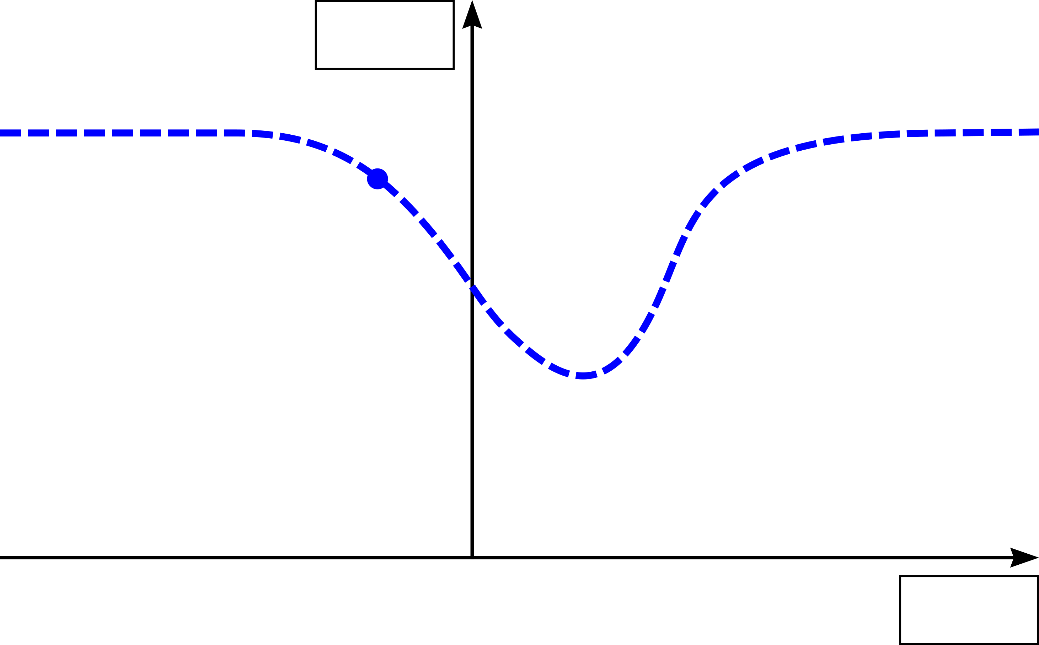
\includegraphics[width=0.66\textwidth]{figures/cv_fig4_blank.png}};
\begin{scope}[x={(img.south east)},y={(img.north west)}]
  \clip (0.0,0.13) rectangle (1.0,0.97);
  \draw[red,dashed,line width=1.1pt] plot coordinates {(0.000,0.795) (0.029,0.795) (0.059,0.795) (0.096,0.795) (0.125,0.794) (0.154,0.788) (0.182,0.777) (0.209,0.759) (0.234,0.729) (0.257,0.705) (0.281,0.671) (0.304,0.622) (0.328,0.572) (0.351,0.517) (0.374,0.478) (0.398,0.445) (0.424,0.423) (0.452,0.420) (0.481,0.455) (0.504,0.505) (0.527,0.586) (0.550,0.665) (0.575,0.716) (0.601,0.743) (0.629,0.763) (0.657,0.775) (0.686,0.784) (0.715,0.789) (0.745,0.793) (0.782,0.795) (0.812,0.795) (0.842,0.795) (0.871,0.796) (1.000,0.796)};
  \draw[green!55!black,dash dot,line width=1.1pt] plot coordinates {(0.000,0.795) (0.030,0.795) (0.059,0.795) (0.089,0.795) (0.119,0.795) (0.156,0.795) (0.185,0.794) (0.214,0.788) (0.242,0.777) (0.269,0.759) (0.294,0.729) (0.317,0.705) (0.341,0.671) (0.364,0.622) (0.388,0.572) (0.411,0.517) (0.434,0.478) (0.458,0.445) (0.484,0.423) (0.512,0.420) (0.541,0.455) (0.564,0.505) (0.587,0.586) (0.610,0.665) (0.635,0.716) (0.661,0.743) (0.689,0.763) (0.717,0.775) (0.746,0.784) (0.775,0.789) (0.805,0.793) (0.842,0.795) (0.872,0.795) (0.902,0.795) (0.931,0.796) (1.000,0.796)};
  \draw[violet,densely dotted,line width=1.1pt] plot coordinates {(0.000,0.795) (0.120,0.795) (0.150,0.795) (0.180,0.795) (0.210,0.795) (0.239,0.795) (0.269,0.795) (0.299,0.795) (0.336,0.795) (0.365,0.794) (0.394,0.788) (0.422,0.777) (0.449,0.759) (0.474,0.729) (0.497,0.705) (0.521,0.671) (0.544,0.622) (0.568,0.572) (0.591,0.517) (0.614,0.478) (0.638,0.445) (0.664,0.423) (0.692,0.420) (0.721,0.455) (0.744,0.505) (0.767,0.586) (0.790,0.665) (0.815,0.716) (0.841,0.743) (0.869,0.763) (0.897,0.775) (0.926,0.784) (0.955,0.789) (0.985,0.793) (1.000,0.793)};
  \draw[red,-{Latex},line width=0.9pt] (0.40,0.66)--(0.31,0.66);
  \draw[violet,-{Latex},line width=0.9pt] (0.62,0.66)--(0.71,0.66);
\end{scope}
\begin{scope}[x={(img.south east)},y={(img.north west)}]
  \node at (0.37,0.915) {\small $C$};
  \node at (0.93,0.05) {\small $V_G$};
\end{scope}
\end{tikzpicture}
